\documentclass[tikz,border=10pt]{standalone}
\usepackage{amsmath}
\usetikzlibrary{shapes,positioning}

\begin{document}

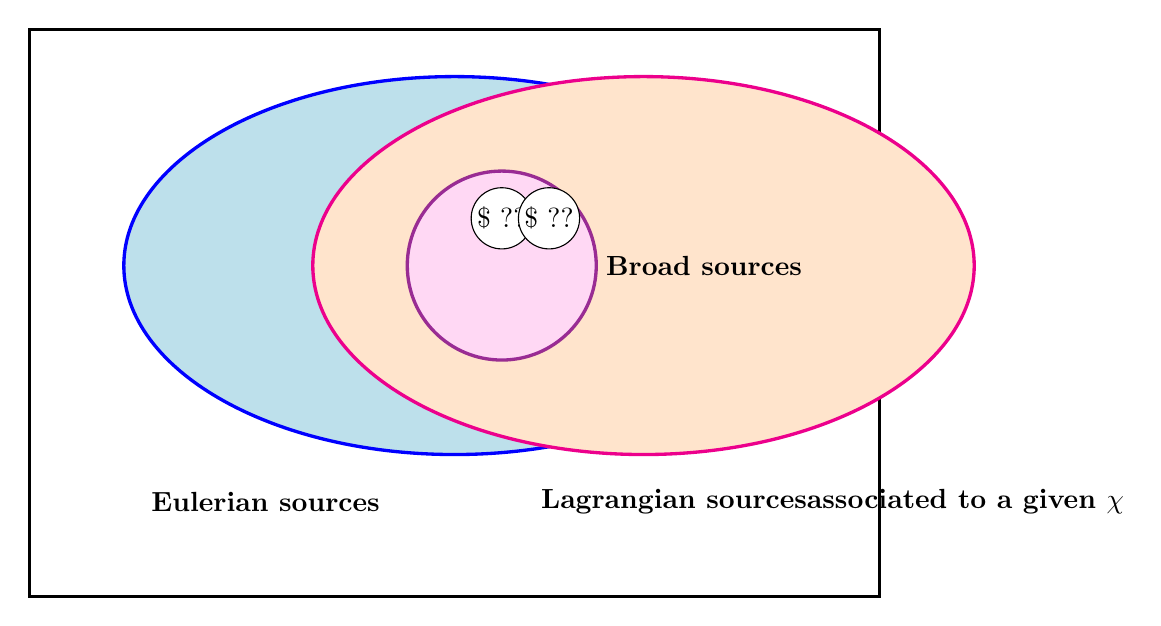
\begin{tikzpicture}[scale=1.2]

% Define colors
\definecolor{eulerian}{RGB}{173, 216, 230} % Light blue
\definecolor{lagrangian}{RGB}{255, 221, 191} % Light orange
\definecolor{intersection}{RGB}{255, 204, 255} % Light purple

% Bounding box for "Borel, bounded functions"
\draw[very thick] (-4.5,-3.5) rectangle (4.5,2.5) node[midway] {\textbf{Borel, bounded functions}};

% Eulerian sources ellipse
\filldraw[fill=eulerian!80, draw=blue, very thick]
  (0,0) ellipse [x radius=3.5, y radius=2];
\node at (-2,-2.5) {\textbf{Eulerian sources}};

% Lagrangian sources ellipse
\filldraw[fill=lagrangian!80, draw=magenta, very thick]
  (2,0) ellipse [x radius=3.5, y radius=2];
\node at (4,-2.5) {\textbf{Lagrangian sources \\ associated to a given \( \chi \)}};

% Intersection region (shaded differently)
\fill[fill=intersection!80, draw=violet, very thick, opacity=0.8]
  (0.5,0) circle [radius=1];

% Labels in the intersection region
\node[circle, fill=white, draw=black, inner sep=1pt] at (0.5,0.5) {\(\$\ ??\)};
\node[circle, fill=white, draw=black, inner sep=1pt] at (1.0,0.5) {\(\$\ ??\)};
\node[right] at (1.5,0) {\textbf{Broad sources}};

% Additional bounding box for clarity (if needed)
% \draw[dashed] (-4.5,-3.5) rectangle (4.5,2.5);

\end{tikzpicture}

\end{document}